% !TEX TS-program = xelatex
% !TEX encoding = UTF-8 Unicode
\documentclass[AutoFakeBold]{MyFormat}

\usepackage{listings}

\lstset{
 columns=fixed,       
 numbers=left,                                        % 在左侧显示行号
 numberstyle=\tiny\color{gray},                       % 设定行号格式
 frame=none,                                          % 不显示背景边框
 backgroundcolor=\color[RGB]{245,245,244},            % 设定背景颜色
 keywordstyle=\color[RGB]{40,40,255},                 % 设定关键字颜色
 numberstyle=\footnotesize\color{darkgray},           
 commentstyle=\it\color[RGB]{0,96,96},                % 设置代码注释的格式
 stringstyle=\rmfamily\slshape\color[RGB]{128,0,0},   % 设置字符串格式
 showstringspaces=false,                              % 不显示字符串中的空格
 language=python,                                        % 设置语言
}

\begin{document}
%=====%
%
%封皮页填写内容
%
%=====%

% 标题样式 使用 \title{{}}; 使用时必须保证至少两个外侧括号
%  如: 短标题 \title{{第一行}},  
% 	      长标题 \title{{第一行}{第二行}}
%             超长标题\tiitle{{第一行}{...}{第N行}}

\title{{FGRMER论文精读}}
\entitle{{Learning Notes From 2022.06.05}}
\author{Sillin Ini\\Pinyi Huang}
\maketitle
\thispagestyle{empty}
\newpage

%生成目录
\tableofcontents
\thispagestyle{empty}
\newpage

%文章主体
\mainmatter




% =======正文从第一章开始
\setcounter{chapter}{0}

\chapter{学习过程中的疑问}
\section{关于GCN传播公式实现的代码}
\par 由矩阵$\tilde A$的求取方法可以知道,在矩阵$\tilde A$中,
$P_{ij}\ne P_{ji}$,即矩阵$\tilde A$并不是对称矩阵。那么根据代码来看,
矩阵运算$(\tilde AD)^TD = (D^T\tilde A^T)D = D\tilde A^TD$是否与原公式不符?
\begin{figure}[!h]
    \centering
    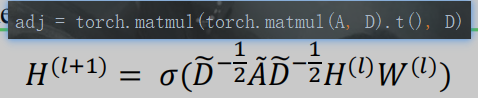
\includegraphics[width=0.6\linewidth]{figures/2022.06.05/ques_GCN.png}
    \caption{上方为官方实现代码,下方为GCN传播公式}
\end{figure}

\section{关于nn.Dropout和nn.ReLU}
\par nn.Dropout和nn.ReLU是可训练的吗?
当所有ReLU和Dropout层参数均相同时,为什么不能整个模型都采用同一个
nn.Dropout和nn.ReLU层,而要分开写?
\par 或者,能不能在需要使用的时候,直接从torch.nn里进行调用?
\begin{figure}[!h]
    \centering
    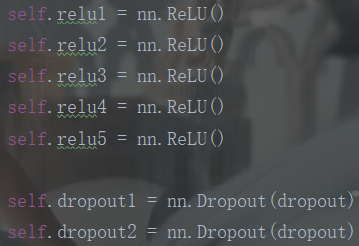
\includegraphics[width=0.4\linewidth]{figures/2022.06.05/ques_relu.png}
\end{figure}


\section{关于神经网络最后的log\_softmax}
\par 既然最后同样是使用了torch.data.max函数来找输出每一行中的最大值,
那么最后的这个log\_softmax步骤是否可以省略?
\begin{lstlisting}[language=python]
    x = torch.cat([part1, part2], dim = 1)
    x = self.layer_norm1(x)
    x = self.linear5(x)
    return F.log_softmax(x, dim=1)
\end{lstlisting}


\section{关于$\tilde A$矩阵}
\par 在GCN的计算公式中:
\begin{equation}
    H^{(l+1)} = \sigma(\tilde D^{-\frac{1}{2}}\tilde A
    \tilde D^{-\frac{1}{2}}H^{(l)}W^{(l)})
\end{equation}
\par 按道理来说$\tilde A$应该是一个不可训练的矩阵,即应该是一个固定的矩阵,
为什么还要使用Parameter()转换为可训练的矩阵?
\par 是因为之后有个detach()阻断了传播,实际上并不会训练吗?
\begin{lstlisting}
    # 这里生成了A = A + In
    _adj = gen_A(9, adj_file)
    self.A = Parameter(torch.from_numpy(_adj).float())
    # 这里生成了归一化后的D^AD^
    adj = gen_adj(self.A).detach()
\end{lstlisting}


\section{关于归一化的问题}
\par 在代码中,既使用了BatchNorm也使用了LayerNorm,这两个归一化函数应该怎样
选择?即何时使用哪一种归一化该如何决定?



\chapter{Introduction总体概述}
\section{关于微表情识别方法的三大类}
\begin{itemize}
    \item 基于LBP的微表情识别方法:在微表情帧之间的变化中,
    其更多的是面部肌肉引起的几何变换。而由于LBP更多注重于纹理信息,
    纹理信息是十分容易受到外部因素干扰的,如环境照明变化、人种等,
    因此LBP算法通常都不是微表情识别的最好方法。
    \item 基于光流的(\textit{Optical-Flow-Based})方法:
    LBP特征通常被称为低级特征,而光流则被称为更高级的特征。
    在深度学习方法被引入MER之前,通常都是采用光流进行特征提取,
    而现在则主要是使用神经网络,如CNN、LSTM、GCN等,
    或他们的变体及组合进行特征提取。
    \item 其他新方法,主要都是基于深度学习。
\end{itemize}
\par 在视频动作增强中,本文使用了基于转换学习的MagNet。
经过该深度学习网络增强后的形状表示是几何特征,因此可以作为
更深层特征提取和学习的输入。
\par 而经过这一次几何特征增强后,这一方法在当时取得了最好的识别率,
这也证明了增强的几何特征对MER有着十足的帮助。


\section{关于点学习(\textit{Node Learning})部分}
\par 由于微表情通常都是面部的微小变化,因此将整个面部照片直接输入进神经网络
是十分粗鲁的,由此需要提取一些特定大小的patches作为输入。
\par 由于之后的边学习中使用到了Encoder,
因此每个patch需要转换成$1\times 49$的形状。
为了在一定程度上保留特征的空间信息,减少因形状拉伸导致的竖直空间信息损失,
需要进行一个“点学习”。
\par 点学习的过程主要步骤如下:
\begin{enumerate}
    \item 首先,从增强后的形状特征中,截取30个patches,
    每个patches的大小为$7\times 7$,具体方法为:在人脸的66个特征点中,
    找出30个与眉毛和嘴巴相关的特征点,在每个特征点周围取相邻的
    $7\times 7$像素区域。这些$30\times 7\times 7$的数据就被称为
    \textbf{\Large \underline{面部图}}。
    \item 然后,将30个patches视为30个channels,将其输入Depthwise CNN进行学习。
    在此过程中,要保持每个patch的形状不变,即仍为$7\times 7$;
\end{enumerate}


\section{关于AU部分}
\par 部分论文中并没有考虑到面部表情可以通过动作单元AU进行编码的机制,
因此考虑AU对MER的影响有着极大的提升空间。
\par 不同的表情类别对应着不同的AU组合,因此AU中包含的信息对MER有帮助。

\section{关于融合Fusion的部分}
\par 在本文中,设计了两条通道进行工作:
\begin{itemize}
    \item 使用神经网络和Encoder对特征进行提取和联系学习的通道;
    \item 对AU信息进行学习的通道,这一部分通过GCN进行学习。
\end{itemize}
\par 最后,两个通道的信息通过一种特定的方式进行融合。



\chapter{论文中提出的方法}


\par 在论文中提出了“一个通道学习面部图表示,另一个通道学习一个动作单元矩阵,
并提出了一个双通道融合的新机制并用于微表情识别”。

\par 一方面,仅采用了每个表情的Onset Frame和Apex Frame输入MagNet,
来从中间层提取增强后的形状特征。然后提取$30\times 7\times 7$的图表示,
并在图表示中进行点学习,之后使用Encoder进行图表示学习。
\par 另一方面,在所有36个AU中,只有9个AU与眉毛和嘴巴区域相关,因此将这9个
区域通过词嵌入和GCN进行学习,并得到\textbf{\Large \underline{AU特征矩阵}}。
\par 最后,使用一个融合机制,将双通道信息融合,并用于微表情分类识别。



\section{点学习(\textit{Node Learning})}

\par 其大致步骤如下:
\begin{itemize}
    \item 首先使用一个深度卷积(\textit{Depthwise Convolution})
    来学习空间特征;
    \item 之后将每个patches拉伸,经过卷积后,这一步中带来的垂直空间
    信息损失,在一定程度上得到了缩减;
    \item 将拉伸后的patches丢入Encoder中学习相互的关联;
    \item 最后分别经过两次全连接层、两次激活层和一次Dropout层进行学习,
    增强神经网络的表示能力。
\end{itemize}


\chapter{关于代码}
\section{Mydataset.py}
\par 这一部分是关于数据的读取。在这一部分中,需要思考如下几个问题来辅助重写:
\begin{itemize}
    \item 构造的MyDataset最终需要使用DataLoader进行数据提取,因此需要
    继承自什么类?
    \item 关于这篇论文,出于测试,需要一些什么参数?
    \item 在构造这个类别时,至少需要自己重载几个函数?分别需要什么参数?
    实现什么功能?
    \item 在读取原始数据的时候,需要使用什么包读取?怎样读取?语法是什么?
    \item 数据怎样被组织?怎样被保存?
\end{itemize}

\section{Transformer.py}
\par 这篇论文中只使用到了Encoder部分,来获取各节点之间的关系,称为边学习。
由此理论上来说,只需要编写Encoder部分即可。
\par 根据以下Encoder的结构图,仔细观察数据的流通方式和模型结构。
\begin{figure}[!h]
    \centering
    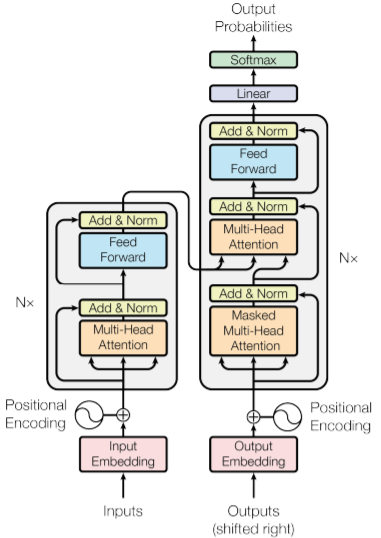
\includegraphics[width=0.4\linewidth]{figures/2022.06.05/Encoder.png}
    \caption{Transformer结构图}
\end{figure}
\par 思考如下几个问题来辅助重写:
\begin{itemize}
    \item Encoder部分需要几个参数?分别代表了什么含义?
    \item Encoder中有几个部分?需要定义几个类?
    \item MultiHeadAttention中有几个部分?需要定义几个层?需要什么参数?
    \item FeedForward中有几个层?需要什么参数?
    \item 关于Encoder的关键算式,需要怎样实现?需要什么参数?
\end{itemize}


\section{Networks.py}
\par 在这一文件中,写的是使用模型的代码。思考如下问题辅助编写:
\begin{itemize}
    \item NetworkModel模型需要几个输入参数?每个参数代表了什么含义?
    \item NetworkModel中包含了几个部分?各自如何实现?
    \item 需要用到几次归一化?需要的参数分别是多少?
    \item 关于面部特征学习通道:
    \begin{itemize}
        \item 按照Linear $\to$ ReLU $\to$ Dropout的顺序来写代码;
        \item 每一次线性变换或卷积变化之后,都需要一次ReLU,
        而是否需要Dropout需要视情况而定;
        \item 深度卷积之后需要使用一次批归一化和ReLU;
        \item 注意何时需要转换形状
    \end{itemize}
    \item 关于AU部分:
    \begin{itemize}
        \item 怎样实现GCN传播公式?各个变量怎样得到?
        \item 每个变量代表了什么含义?怎样实现?
        \item 在这一部分使用了什么激活函数?参数是多少?
        \item 怎样初始化参数?有几处?
    \end{itemize}
    \item 关于融合部分:
    \begin{itemize}
        \item 怎样实现融合?
        \item 融合以后怎样输出?
    \end{itemize}
\end{itemize}


\section{utils.py}
\par 在这个文件中,实现了两个函数,其分别对应于求GCN中的两个矩阵:
$\tilde A$和$\tilde D^{-\frac{1}{2}}\tilde A\tilde D^{-\frac{1}{2}}$。


\section{FGRMER\_run.py}
\par 在这个文件中,实现了各个模块的运行和流程的控制。
\par 注意在过程中需要将模型转移到GPU上,并使用测试模式。







\end{document}